% Jacob Neumann

% DOCUMENT CLASS AND PACKAGE USE
    \documentclass[aspectratio=169]{beamer}
 
    % Establish the colorlambda boolean, to control whether the lambda is solid color (true), or the same as the picture (false)
    \newif\ifcolorlambda
    \colorlambdafalse % DEFAULT: false
    
    % Use auxcolor for syntax highlighting
    \newif\ifuseaux
    \useauxfalse % DEFAULT: false
   
    % Color settings
    \useauxtrue
    
    \newcommand{\auxColor}{B109CC}     % the color of note boxes and stuff
    \newcommand{\presentColor}{FF3364} % the primary color of the slide borders
    \newcommand{\bgColor}{fff0f4}      % the color of the background of the slide
    \newcommand{\darkBg}{8b98ad}
    \newcommand{\lambdaColor}{\auxColor}
  
    \colorlambdatrue

    \usepackage{comment} % comment blocks
    \usepackage{soul} % strikethrough
    \usepackage{listings} % code
    \usepackage{makecell}

    \usepackage{tikz} % Import the tikz package
    \usetikzlibrary{automata} 
    \usetikzlibrary{positioning} 
    \usetikzlibrary{arrows} 
    \usetikzlibrary{decorations.pathreplacing,calligraphy}

    \tikzset{node distance=2.5cm, % Minimum distance between two nodes. Change if necessary.
      every state/.style={ % Sets the properties for each state
      semithick,
      fill=gray!10},
      initial text={}, % No label on start arrow
      double distance=2pt, % Adjust appearance of accept states
      every edge/.style={ % Sets the properties for each transition
            draw,
      ->,>=stealth', % Makes edges directed with bold arrowheads
      auto,
      semithick}}

    \setbeamertemplate{itemize items}[circle]
    % \setbeameroption{show notes on second screen=right}

    \usepackage{lectureSlides}
    %%%%%%%%%%%%%%%%%%%%%%%%%%%%%%%%%%%%%%%%%| <----- Don't make the title any longer than this
    \title{Regular Expressions} % TODO
    \subtitle{Finding patterns in text} % TODO
    \date{03 July 2023} % TODO
    \author{Brandon Wu} % TODO

    \graphicspath{ {./img/} }
    % DONT FORGET TO PUT [fragile] on frames with codeblocks, specs, etc.
        %\begin{frame}[fragile]
        %\begin{codeblock}
        %fun fact 0 = 1
        %  | fact n = n * fact(n-1)
        %\end{codeblock}
        %\end{frame}

    % INCLUDING codefile:
        % 1. In some file under code/NN (where NN is the lecture id num), include:
    %       (* FRAGMENT KK *)
    %           <CONTENT>
    %       (* END KK *)
    
    %    Remember to not put anything on the same line as the FRAGMENT or END comment, as that won't be included. KK here is some (not-zero-padded) integer. Note that you MUST have fragments 0,1,...,KK-1 defined in this manner in order for fragment KK to be properly extracted.
        %  2. On the slide where you want code fragment K
                % \smlFrag[color]{KK}
        %     where 'color' is some color string (defaults to 'white'. Don't use presentColor.
    %  3. If you want to offset the line numbers (e.g. have them start at line 5 instead of 1), use
                % \smlFragOffset[color]{KK}{5}

\begin{document}

% Make it so ./mkWeb works correctly
\ifweb
    \renewcommand{\pause}{}
\fi

\setbeamertemplate{itemize items}[circle]

% SOLID COLOR TITLE (see SETTINGS.sty)
{
\begin{frame}[plain]
    \colorlambdatrue
    \titlepage
\end{frame}
}

\menti{2955 1356}

\begin{frame}[fragile]
  \frametitle{Lesson Plan}

  \tableofcontents
\end{frame}

\sectionSlide{1}{Text Validation}

\begin{frame}[fragile]
  \frametitle{Reading Emails}

  Suppose that we are interested in the problem of validating user input.

  \pause
  \vspace{\fill}

  In this particular circumstance, assume that we are taking input that is
  supposed to look like an email. We expect an input which looks something like
  $$\langle name \rangle\textsf{@}\langle website\rangle\textsf{.}\langle extension \rangle$$

  \pause
  \vspace{\fill}

  \spec
    {validateEmail}
    {string -> bool}
    {\code{true}}
    {\code{validateEmail s} $\stepsTo^*$ \code{true} iff \code{s} is a valid 
    email address}
\end{frame}

\begin{frame}[fragile]
  \frametitle{Reading Emails}

  \rprs

  We note that this problem can be solved by noticing what characters fall into
  each section of the email. We know that \code{@} and \code{.} need to show
  up, but there are different requirements for the name, website, and extension!

  \pause
  \vspace{\fill}

  For simplicity, we assume that:
  \pause
  \begin{itemize}
    \item an $\langle extension\rangle$ can only be "org" or "com" \pause
    \item a $\langle website\rangle$ must be fully alphanumeric \pause
    \item a $\langle name\rangle$ must be fully alphanumeric, plus underscores and periods
  \end{itemize}

  \pause
  \vspace{\fill}

  To facilitate our implementation of \code{validateEmail}, we will define a series
  of \term{consumer} functions, which simply serve to consume each of the constituent
  email parts from the front of a list of characters.
\end{frame}

\begin{frame}[fragile]
  \frametitle{Consuming Input}

  \spec
    {consumeName}
    {char list -> char list}
    {\code{true}}
    {\code{consumeName cs} evaluates to the suffix of \code{cs} caused by
    removing all characters that could be in a $\langle name\rangle$}

  \vspace{\fill}

  \spec
    {consumeWebsite}
    {char list -> char list}
    {\code{true}}
    {\code{consumeWebsite cs} evaluates to the suffix of \code{cs} caused by
    removing all characters that could be in a $\langle website\rangle$}
\end{frame}


\begin{frame}[fragile]
  \frametitle{Consuming Input}

  \pause
  \small
  \begin{codeblock}
    fun consumeName [] = [] 
      | consumeName (c::cs) =
          if Char.isAlphaNum c then
            consumeName cs 
          else
            case c of
              #"." => consumeName cs
            | #"_" => consumeName cs
            | _ => c::cs
  \end{codeblock}

  \begin{codeblock}
    fun consumeWebsite [] = [] 
      | consumeWebsite (c::cs) =
          if Char.isAlphaNum c then
            consumeWebsite cs 
          else
            c::cs
  \end{codeblock}
\end{frame}

\begin{frame}[fragile]
  \frametitle{Validating Emails}

  \pause
  \begin{codeblock}
    fun validateEmail s = 
      case consumeName (String.explode s) of
        #"@"::cs =>
          (case consumeWebsite cs of
            #"."::#"o"::#"r"::#"g"::_ => true
          | #"."::#"c"::#"o"::#"m"::_ => true
          | _ => false
          )
      | _ => false 
  \end{codeblock}

  \pause
  \vspace{\fill}

  Sounds good, right?
\end{frame}

\begin{frame}[fragile]
  \frametitle{Validating Emails}

  No, actually. There's a bug with our code: 

  \pause
  \begin{codeblock}
    fun validateEmail s = 
      case validateName (String.explode s) of
        #"@"::cs =>
          (case validateWebsite cs of
            `[#".", #"o", #"r", #"g"]` => true
          | `[#".", #"c", #"o", #"m"]` => true
          | _ => false
          )
      | _ => false 
  \end{codeblock}
  %'

  \pause
  \vspace{\fill}

  We need to make sure that the extension is the last thing in the
  email!

  \pause
  \vspace{\fill}

  How about now?
\end{frame}

\begin{frame}[fragile]
  \frametitle{Handrolling}

  The above is what we would term a \term{hand-rolled} function.

  \pause
  \vspace{\fill}

  This is because it's manually constructed, tedious, and as we will
  see, more easily solvable in a way that doesn't involve coding a solution
  from scratch. Hand-rolling is usually undesirable, because more handwritten
  code means more possibility of errors. 

  \pause
  \vspace{\fill}

  \customBox{Mantra}{\, \textbf{More code, more problems.}}

  \pause
  \vspace{\fill}

  This same logic can apply to many situations. For instance, we might be
  interested in validation for strings which look like home addresses,
  or strings which look like filenames of images, or strings which are valid
  social security numbers.

  \pause
  \vspace{\fill}

  Can we somehow find a way to automate the boilerplate process of writing
  code like this?
\end{frame}

\begin{frame}[fragile]
  \frametitle{A Family of Validators}

  Essentially, we are looking for a family of functions, which would have
  type \code{t -> string -> bool}. This type \code{t} would need to be able
  to encode the information of the entire form of one of these validation functions,
  such as \code{validateEmail}, which could then be given as input to produce the
  validation function itself.

  \pause
  \vspace{\fill}

  In essence, we are looking for \textit{the} "essence" of a string validation problem.

  \pause
  \vspace{\fill}

  This type \code{t} will end up being the type of \term{regular expressions}.
\end{frame}

\sectionSlide{2}{Regular Expressions}

\begin{frame}[fragile]
  \frametitle{On Regular Expressions}

  \begin{center}
    \includegraphics[scale=0.35]{regex1}
  \end{center}
\end{frame}

\begin{frame}[fragile]
  \frametitle{On Regular Expressions}

  \begin{center}
    \includegraphics[scale=0.7]{regex2}\footnotemark
  \end{center}

  \footnotetext[1]{There's an xkcd for everything.}
\end{frame}

\begin{frame}[fragile]
  \frametitle{On Regular Expressions}

  PCRE, which stands for Perl Compatible Regular Expressions, is a particular
  library and syntax for regular expressions, which allow us to solve certain
  string matching problems.

  \pause
  \vspace{\fill}

  We'll take the PCRE, and cut out the PC. We don't have time for that.

  \pause
  \vspace{\fill}

  At the end of this lecture, you will not know how to actually use regular
  expressions in the real world, but you will know how they work. 
  That's the important part.
\end{frame}



\begin{frame}[fragile]
  \frametitle{Essential Elements}

  \rprs

  What are the essential elements that make up a "validator"? Recall the email
  example we were just looking at. There's a few important things that we should
  be able to do: 

  \pause
  \begin{itemize}
    \item Concatenation - Match one pattern, and then another. For instance,
    matching the name and then the \code{@} symbol. \pause
    \item Alternation - Match possibly one of two patterns. For instance, we
    could match \textit{either} \code{org} or \code{com} at the end. \pause
    \item Iteration - Match one pattern, as much as you can. For instance,
    to match a website, we needed to be able to match an alphanumeric character any
    number of times. 
  \end{itemize}

  \pause
  \vspace{\fill}

  This sure seems like a recursive definition.
\end{frame}

\begin{frame}[fragile]
  \frametitle{Mathematical Notation}

  \ptmt

  Having now described the problem, let's describe the mathematical definition
  of a regular expression.

  \pause
  \vspace{\fill}

  \defBox{}{\, We say that an \term{alphabet} is a set of characters, that we
  are interested in strings composed from. We usually denote this symbolically
  as $\Sigma$.}

  \pause
  \vspace{\fill}

  So for instance, we could have that $\Sigma = \{a, b\}$. Usually, our
  alphabet of interest will simply be the alphabet of English letters.

  \pause
  \vspace{\fill}

  \defBox{}{\, We denote the set of strings over an alphabet $\Sigma$ by the
  symbol $\Sigma^*$.}

  \pause
  \vspace{\fill}

  In this case, then we would have that \code{"abaa"} $\in \Sigma^*$.
\end{frame}

\begin{frame}[fragile]
  \frametitle{More Mathematical Notation}

  \defBox{}{\, We say that a \term{language} $L$ is a subset of $\Sigma^*$. In
  other words, a language is a particular set of strings composed from the 
  alphabet $\Sigma$.}

  \pause
  \vspace{\fill}

  So we might say that some examples of languages over $\Sigma = \{a, b\}$ are
  the empty set, $\{a, aa, aaa, ...\}$, $\{b, bb, bbb, ...\}$, 
  and $\{a, bb\}$. 

  \pause
  \vspace{\fill}

  When we say "string", we mean any finite-length sequence of characters from
  an alphabet. This includes a string of length 0, which is really hard to
  write out. As such, as will notate the empty string as $\epsilon$.
\end{frame}

\begin{frame}[fragile]
  \frametitle{Validators and Regular Expressions}

  Viewed in this notation, what is a validator?

  \pause
  \vspace{\fill}

  A validator is simply a function which checks for membership within a
  language. For instance, our \code{validateEmail} function is simply a
  function that checks if a string is present in the language of all emails,
  with emails defined as we said previously.

  \pause
  \vspace{\fill}

  \defBox{}{\, We call a function \code{f : string -> bool} a \term{validator} 
  for language $L$, if \\ \code{f s} $\stepsTo^*$ \code{true} iff $s \in L$.\footnotemark}

  \pause
  \vspace{\fill}
  
  We will find that \term{regular expressions} allow us to implement
  validators for a class of languages called \term{regular languages}. These
  have limitations on their complexity, but in practice a large amount
  of string validation problems fall into them. 

  \footnotetext[2]{
   As an aside, this idea of languages and validators over them is very closely tied to
  the idea of computability! In particular, it is \textbf{not} possible, 
  for every language $L$, to implement a validator for it. A more thorough treatment of this is reserved for a class on
  computability theory, such as 15-251.}
\end{frame}

\begin{frame}[fragile]
  \frametitle{The Structure of a Regular Expression}

  \defBox{}{\, Let's first define the structure of a regular expression $r$:}

  \pause
  \begin{itemize}
    \item $0$
    \item $1$ \pause
    \item $c$, for any character $c \in \Sigma$ \pause
    \item $r_1 + r_2$, for two regular expressions $r_1$ and $r_2$
    \item $r_1r_2$, for two regular expressions $r_1$ and $r_2$
    \item $r*$, for a regular expression $r$
  \end{itemize}

  \pause
  \vspace{\fill}

  If this looks to you like a datatype declaration, that's because soon
  it will be.
\end{frame}

\begin{frame}[fragile]
  \frametitle{The Language of a Regular Expression}

  \defBox{}{\, We use the notation $L(r)$ to denote the language matched by
  regular expression $r$, over some alphabet $\Sigma$. Then:}

  \pause
  \begin{center}
    \begin{tabular}{c || c} 
      \hline & \\[-1.5ex]
      Construct & Language matched \\ [2pt]
      \hline & \\[-2ex]
      \hline & \\[-1.5ex]
      $L(c)$ & $\{ c \}$ \\ [2pt]
      \hline & \\[-1.5ex]
      $L(0)$ & $\{ \}$ \\ [2pt]
      \hline & \\[-1.5ex]
      $L(1)$ & $\{ \epsilon \}$ \\ [2pt]
      \hline & \\[-1.5ex]
      $L(r_1 + r_2)$ & $L(r_1) \cup L(r_2)$ \\ [2pt]
      \hline & \\[-1.5ex]
      $L(r_1r_2)$ & $\{ s_1s_2 \, | \, s_1 \in L(r_1),\, s_2 \in L(r_2) \}$ \\ [2pt]
      \hline & \\[-1.5ex]
      $L(r^*)$ & $\{ s_1 ... s_n \,\, | \,\, \text{for } n \geq 0, \text{when } \forall i, s_i \in L(r) \}$ \\ [2pt]
      \hline
    \end{tabular}
  \end{center}
\end{frame}

\begin{frame}[fragile]
  \frametitle{The Language of a Regular Expression, In English}

  \begin{center}
    \begin{tabular}{c || c} 
      \hline & \\[-1.5ex]
      Construct & Matches \\ [2pt]
      \hline & \\[-2ex]
      \hline & \\[-1.5ex]
      $L(c)$ & only $c$ \\ [2pt]
      \hline & \\[-1.5ex]
      $L(0)$ & nothing \\ [2pt]
      \hline & \\[-1.5ex]
      $L(1)$ & only the empty string \\ [2pt]
      \hline & \\[-1.5ex]
      $L(r_1 + r_2)$ & anything matched by either $r_1$ or $r_2$ \\ [2pt]
      \hline & \\[-1.5ex]
      $L(r_1r_2)$ & anything with a prefix matched by $r_1$ and suffix matched by $r_2$ \\ [2pt]
      \hline & \\[-1.5ex]
      $L(r^*)$ & any string which is something matched by $r$, 0 or more times \\ [2pt]
      \hline
    \end{tabular}
  \end{center}
\end{frame}

\begin{frame}[fragile]
  \frametitle{Regular Expression Examples}

  Let's look at some examples of regular expressions and the languages they match.

  \vspace{\fill}

  In this example, let's assume we are working with the alphabet $\Sigma = \{a, b\}$.

  \pause
  \vspace{\fill}

  \begin{center}
    \begin{tabular}{c || c} 
      \hline & \\[-1.5ex]
      Regular Expression & Language matched \\ [2pt]
      \hline & \\[-2ex]
      \hline & \\[-1.5ex]
      $a + b$ & $\{a, b\}$ \\ [2pt]
      \hline & \\[-1.5ex]
      $abaa + baa$ & $\{abaa, baa\}$ \\ [2pt]
      \hline & \\[-1.5ex]
      $(abaa + baa)b$ & $\{ abaab, baab \}$ \\ [2pt]
      \hline & \\[-1.5ex]
      $0 + a$ & $\{a\}$ \\ [2pt]
      \hline & \\[-1.5ex]
      $1 + a$ & $\{ \epsilon, a \}$ \\ [2pt]
      \hline & \\[-1.5ex]
      $a^*$ & $\{ \epsilon, a, aa, aaa, aaaa, ... \}$ \\ [2pt]
      \hline
    \end{tabular}
  \end{center}
\end{frame}

\begin{frame}[fragile]
  \frametitle{On Formalism}

  Let's ground ourselves a little bit. Why are we talking about this?

  \pause
  \vspace{\fill}

  Regular expressions are a useful formalism that allow us to symbolically
  specify certain languages. They are composable, since we can easily form
  regular expressions out of other ones. We haven't yet
  specified how to turn this formalism into code that runs, but this is
  the model by which we will design our code.

  \pause
  \vspace{\fill}

  In particular, recall the website example that we were talking about
  previously. We can express our website validator by the following
  regular expression:
  $${(r_{an} + . + \_ )}^* @ ({r_{an}}^*) . (org + com)\footnotemark$$
  where $r_{an}$ is the regular expression of all alphanumeric 
  characters, which could be specified as $a + b + ... + z + 1 + 2 + ... + 9 + 0$.

  \footnotetext[3]{This is actually not quite it, because this regular expression
  allows an empty name or website. But for the sake of brevity, we'll go with this.}
\end{frame}

\sectionSlide{3}{Finite-State Automata}

\begin{frame}[fragile]
  \frametitle{Regular Expressions and Automata}

  It is a very interesting fact that regular expressions can be viewed as
  \term{finite-state machines}, which are graph-like constructs with \term{states}, 
  which change upon receiving characters as input. In particular, we can 
  characterize them by \term{deterministic finite-state automata}.\footnotemark

  \pause
  \vspace{\fill}

  For instance, here is a finite-state machine corresponding to the regex $ab + ba$:

  \pause
  \vspace{\fill}

  \makebox[\textwidth][c]{
    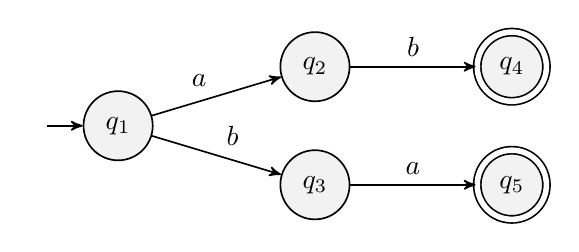
\begin{tikzpicture}
      \node[state, initial] (q1) {$q_1$};
      \node[state, right of=q1, above=0.3cm] (q2) {$q_2$};
      \node[state, right of=q1, below=0.3cm] (q3) {$q_3$};
      \node[state, accepting, right of=q2] (q4) {$q_4$};
      \node[state, accepting, right of=q3] (q5) {$q_5$};
      \draw (q1) edge node {$a$} (q2);
      \draw (q1) edge node {$b$} (q3);
      \draw (q2) edge node {$b$} (q4);
      \draw (q3) edge node {$a$} (q5);
    \end{tikzpicture}
  }

  \footnotetext[4]{We can characterize them by \textbf{nondeterministic} finite-state automata
  as well. But this, too, will be left in more detail to a class on computability.}
\end{frame}

\begin{frame}[fragile]
  \frametitle{The Anatomy of Automata}

  \makebox[\textwidth][c]{
    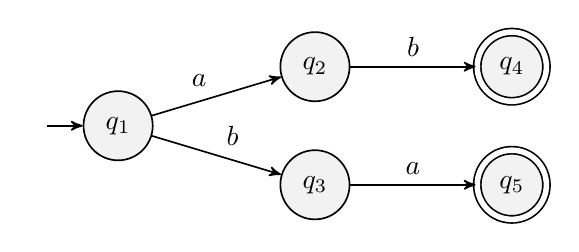
\begin{tikzpicture}
      \node[state, initial] (q1) {$q_1$};
      \node[state, right of=q1, above=0.3cm] (q2) {$q_2$};
      \node[state, right of=q1, below=0.3cm] (q3) {$q_3$};
      \node[state, accepting, right of=q2] (q4) {$q_4$};
      \node[state, accepting, right of=q3] (q5) {$q_5$};
      \draw (q1) edge node {$a$} (q2);
      \draw (q1) edge node {$b$} (q3);
      \draw (q2) edge node {$b$} (q4);
      \draw (q3) edge node {$a$} (q5);
    \end{tikzpicture}
  }

  \pause
  \vspace{\fill}

  Here, we denote the \term{starting state} by the state with an unlabeled 
  in-arrow. 
  
  \pause
  \vspace{\fill}

  From a given state, transitions to other states upon reading a 
  particular character are denoted by arrows labeled with characters. If there 
  is no arrow corresponding to the input character, then the entire string is rejected.

  \pause
  \vspace{\fill}

  We also say that a state is an \term{accepting state} if it is a node which
  has a circle in it. If the state reached upon reading the entire input is an
  accepting state, then we say that that string is in accepted by the FSM.
\end{frame}

\begin{frame}[fragile]
  \frametitle{The Anatomy of Automata}

  Let's try giving this DFA an input, namely the string $ab$.

  \vspace{\fill}

  \makebox[\textwidth][c]{
    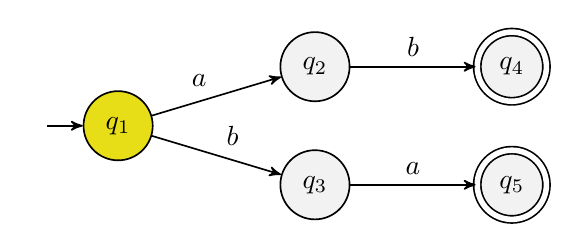
\begin{tikzpicture}
      \node[state, initial, fill=black!10!yellow] (q1) {$q_1$};
      \node[state, right of=q1, above=0.3cm] (q2) {$q_2$};
      \node[state, right of=q1, below=0.3cm] (q3) {$q_3$};
      \node[state, accepting, right of=q2] (q4) {$q_4$};
      \node[state, accepting, right of=q3] (q5) {$q_5$};
      \draw (q1) edge node {$a$} (q2);
      \draw (q1) edge node {$b$} (q3);
      \draw (q2) edge node {$b$} (q4);
      \draw (q3) edge node {$a$} (q5);
    \end{tikzpicture}
  }

  Remaining input: $ab$
\end{frame}

\begin{frame}[fragile]
  \frametitle{The Anatomy of Automata}

  After reading $a$:

  \vspace{\fill}

  \makebox[\textwidth][c]{
    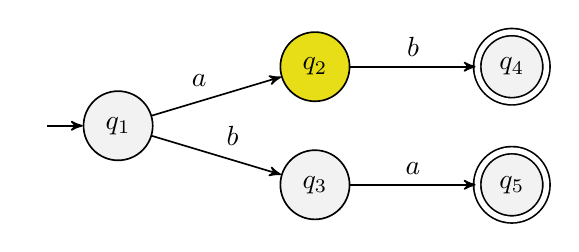
\begin{tikzpicture}
      \node[state, initial] (q1) {$q_1$};
      \node[state, right of=q1, above=0.3cm, fill=black!10!yellow] (q2) {$q_2$};
      \node[state, right of=q1, below=0.3cm] (q3) {$q_3$};
      \node[state, accepting, right of=q2] (q4) {$q_4$};
      \node[state, accepting, right of=q3] (q5) {$q_5$};
      \draw (q1) edge node {$a$} (q2);
      \draw (q1) edge node {$b$} (q3);
      \draw (q2) edge node {$b$} (q4);
      \draw (q3) edge node {$a$} (q5);
    \end{tikzpicture}
  }

  Remaining input: $b$
\end{frame}

\begin{frame}[fragile]
  \frametitle{The Anatomy of Automata}

  After reading $b$:

  \vspace{\fill}

  \makebox[\textwidth][c]{
    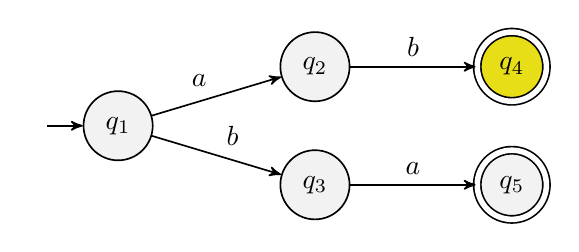
\begin{tikzpicture}
      \node[state, initial] (q1) {$q_1$};
      \node[state, right of=q1, above=0.3cm] (q2) {$q_2$};
      \node[state, right of=q1, below=0.3cm] (q3) {$q_3$};
      \node[state, accepting, right of=q2, fill=black!10!yellow] (q4) {$q_4$};
      \node[state, accepting, right of=q3] (q5) {$q_5$};
      \draw (q1) edge node {$a$} (q2);
      \draw (q1) edge node {$b$} (q3);
      \draw (q2) edge node {$b$} (q4);
      \draw (q3) edge node {$a$} (q5);
    \end{tikzpicture}
  }

  No remaining input, so we end up in state $q_4$, which is accepting. 

  \vspace{\fill}
  
  So the string $ab$ is accepted by this DFA.
\end{frame}

\begin{frame}[fragile]
  \frametitle{Another Regular Expression Automaton}

  Here's another DFA for the regular expression $a^*bba^*$:

  \vspace{\fill}

  \makebox[\textwidth][c]{
    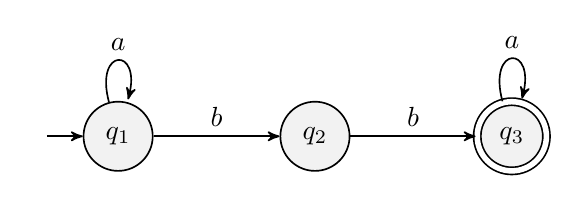
\begin{tikzpicture}
      \node[state, initial] (q1) {$q_1$};
      \node[state, right of=q1] (q2) {$q_2$};
      \node[state, accepting, right of=q2] (q3) {$q_3$};
      \draw (q1) edge[loop above] node {$a$} (q1);
      \draw (q1) edge node {$b$} (q2);
      \draw (q2) edge node {$b$} (q3);
      \draw (q3) edge[loop above] node {$a$} (q3);
    \end{tikzpicture}
  }

  \pause
  \vspace{\fill}

  You should be able to convince yourself that this automaton accepts
  all strings which contain any number of $a$s enclosing two $b$s.
\end{frame}

\quizBreak{BREVITY}

\sectionSlide{4}{Matching Regular Expressions}

\begin{frame}[fragile]
  \frametitle{On the Hardness of DFAs}

  We've seen that, using the DFA for a regular expression, we can
  visualize a computational process for validating strings within a
  particular language.

  \pause
  \vspace{\fill}

  This process is an extremely beautiful intersection where theory and
  practice coincide, and is how many production regular expression engines\footnotemark 
  \, work today. However, the process of producing such an automaton from
  a regular expression is rather involved. We will take another track
  for how to produce a validator from a regular expression.

  \footnotetext[5]{https://github.com/google/re2}
\end{frame}

\begin{frame}[fragile]
  \frametitle{A Type for Regular Expressions}

  \tgs

  We notice that regular expressions are a recursive datatype -- that is,
  regular expressions are composed out of regular expressions.

  \vspace{\fill}

  We can define the type of regular expressions as follows:

  \begin{codeblock}
    datatype regexp = 
        Zero
      | One
      | Char of char  
      | Plus of regexp * regexp
      | Times of regexp * regexp
      | Star of regexp
  \end{codeblock}
\end{frame}

\begin{frame}[fragile]
  \frametitle{Decomposing Regular Expressions}

  \rprs

  The definition of the language of a regular expression is a straightforward
  recursive definition, which depends on the language of the regular sub-expressions.
  Let's try to write a function which can recursively decompose on a regular
  expression, and in a backtracking way, try to match a string.

  \pause
  \vspace{\fill}

  We will find that this is a good application of CPS. We will implement a 
  function:
  \spec
    {match}
    {regexp -> char list -> (char list -> bool) -> bool}
    {\code{k} is total}
    { \\
      \code{match r s k} $\eeq$
    $\left\{
      \begin{array}{lr}
          \code{true}, & \text{if } \code{cs} \eeq \code{p @ s} \text{ where } 
          \code{p} \in L(r) \text{ and } \code{k s} \eeq \code{true} \\
          \code{false}, & \text{otherwise}
      \end{array}
    \right\}
    $
    }
\end{frame}

\begin{frame}[fragile]
  \frametitle{A Special Specification}

  This specification is kind of complicated. Can we desugar it at all?

  \pause
  \vspace{\fill}

  We will find that this type makes our implementation a lot simpler. 
  We use a continuation, specific to return type \code{bool}, to denote 
  a \textit{future condition} we are placing upon the rest of the character
  list. This is useful for branching possibilities, because it lets us enforce a 
  future condition on potentially many suffixes that we might choose to
  consume input to obtain. 

  \pause
  \vspace{\fill}

  For instance, we might be interested in something which looks like
  \code{match r cs (fn cs' => List.length cs' = 3)}.

  \pause
  \vspace{\fill}

  This essentially is a nondeterministic search over \textit{all possible prefixes}
  that can be taken by \code{match}, by the regex \code{r}, \textit{provided} that 
  the suffix to that prefix is of length 3. We change the continuation in order 
  to enforce a condition on all of the possibilities we might pick.
\end{frame}

\begin{frame}[fragile]
  \frametitle{A Visual Specification}

  \begin{center}
    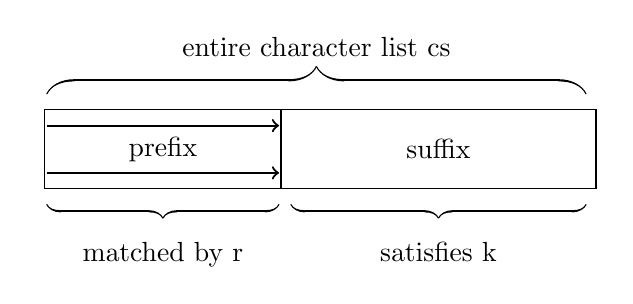
\begin{tikzpicture}
      \node[rectangle, draw=black, minimum height=1cm, minimum width=3cm] (L) {prefix};
      \node[right of=L, rectangle, draw=black, node distance=3.5cm, minimum width=4cm, minimum height=1cm] (R) {suffix};

      \node[above of=L, xshift=-1.6cm, yshift=-1.8cm] (TL) {};
      \node[above of=R, xshift=2cm, yshift=-1.8cm] (TR) {};

      \node[below of=L, xshift=-1.6cm, yshift=2.8cm] (IL) {};
      \node[below of=R, xshift=-1.9cm, yshift=2.8cm] (IR) {};
      \node[below of=L, xshift=-1.6cm, yshift=2.2cm] (IL2) {};
      \node[below of=R, xshift=-1.9cm, yshift=2.2cm] (IR2) {};

      \node[below of=L, xshift=-1.6cm, yshift=1.8cm] (UL) {};
      \node[below of=R, xshift=-1.9cm, yshift=1.8cm] (UR) {};
      \node[below of=L, xshift=1.5cm, yshift=1.8cm] (UL2) {};
      \node[below of=R, xshift=2cm, yshift=1.8cm] (UR2) {};
      \draw[-to, draw=black, thick] (IL) -- (IR);
      \draw[-to, draw=black, thick] (IL2) -- (IR2);
      \draw[thick, decorate, decoration={calligraphic brace, mirror, amplitude=5pt}] (UL) -- (UR)
        node[pos=0.5, below=10pt, black]{matched by \code{r}}
      ;
      \draw[thick, decorate, decoration={calligraphic brace, mirror, amplitude=5pt}] (UL2) -- (UR2)
        node[pos=0.5, below=10pt, black]{satisfies \code{k}}
      ;
      \draw[thick, decorate, decoration={calligraphic brace, amplitude=10pt}] (TL) -- (TR)
        node[pos=0.5, above=10pt, black]{entire character list \code{cs}}
      ;
    \end{tikzpicture}
  \end{center}

  \vspace{\fill}

  Note that the prefix goes from left to right, as we gradually take off more and more
  of the character list, trying out prefixes to see if they will eventually work.
\end{frame}

\begin{frame}[fragile]
  \frametitle{\code{match}: Outline}

  \begin{codeblock}
    fun match (r : regexp) (cs : char list) (k : char list -> bool) : bool =
      case r of
        Zero => (* ... *) 
      | One => (* ... *) 
      | Char c => (* ... *) 
      | Plus (r1,r2) => (* ... *) 
      | Times (r1, r2) => (* ... *) 
      | Star r => (*... *)
  \end{codeblock}
\end{frame}

\begin{frame}[fragile]
  \frametitle{\code{match}: Special Cases}

  Let's write the cases for \code{Zero} and \code{One} first.

  \pause
  \vspace{\fill}

  We know that \code{Zero} matches the empty language, so there is no possible
  prefix that we can take. So we must reject.

  \begin{codeblock}
    Zero => false
  \end{codeblock}

  \pause
  \vspace{\fill}

  For \code{One}, we only allow the empty string. So our prefix must necessarily
  be empty, meaning that the only way to return true is if the entire list satisfies
  the continuation.

  \begin{codeblock}
    | One => k cs
  \end{codeblock}
\end{frame}

\begin{frame}[fragile]
  \frametitle{\code{match}: Characters}

  For the \code{Char} case, we can actually start to take inputs
  off from the list. We know that for the regexp \code{Char c}, the only
  string in that language is \code{c}, so the only prefix we can take is
  the singleton list \code{c}.

  \pause
  \vspace{\fill}

  So we write:

  \begin{codeblock}
    | Char c => (case cs of
        [] => false
      | c' :: cs' => c = c' andalso k cs')
  \end{codeblock}

  because in the empty case, there is no such prefix, and in the cons case,
  we still need to make sure the suffix satisfies the continuation.
\end{frame}

\begin{frame}[fragile]
  \frametitle{\code{match}: Alternation}

  What about the \code{Plus (r1, r2)} case? Here, we have the possibility of
  picking a prefix from either \code{r1} or \code{r2}.

  \pause
  \vspace{\fill}

  Thankfully, the return type of our function \code{match} is just \code{bool},
  and we're not required to write \code{match} tail recursively, so we can
  simply use two recursive calls:

  \begin{codeblock}
    | Plus (r1,r2) => match r1 cs k orelse match r2 cs k
  \end{codeblock}

  \pause
  \vspace{\fill}

  We are essentially searching over all the strings matched by \code{r1} and
  \code{r2} separately, but with the same suffix condition needing to be true.
  Either succeeding means that we succeed in general.
\end{frame}

\begin{frame}[fragile]
  \frametitle{\code{match}: Concatenation}

  For concatenation, we need to be able to pick a prefix from the \code{cs}
  for the first regexp \code{r1}, but then pick another prefix after that for
  \code{r2}.

  \pause
  \vspace{\fill}

  This is exactly the same as looking for a prefix of \code{cs}, but then
  looking for a prefix of the corresponding suffix. Let's write it:

  \begin{codeblock}
    | Times (r1, r2) => match r1 cs (fn cs' => match r2 cs' k)
  \end{codeblock}

  \pause

  \begin{center}
    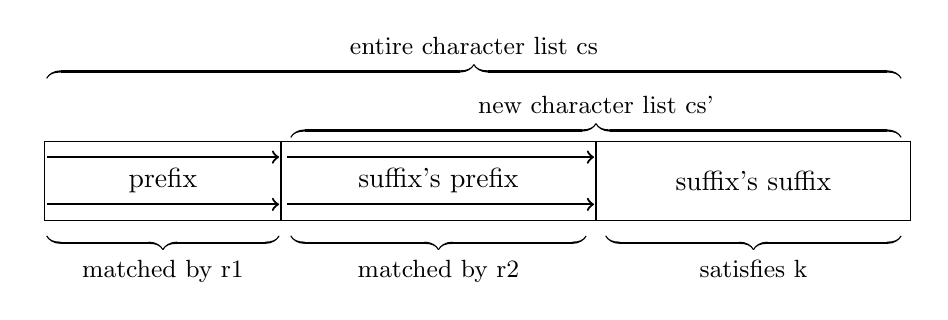
\begin{tikzpicture}
      \node[rectangle, draw=black, minimum height=1cm, minimum width=3cm] (L) {prefix};
      \node[right of=L, rectangle, draw=black, node distance=3.5cm, minimum width=4cm, minimum height=1cm] (R) {suffix's prefix};
      \node[right of=R, xshift=0.5cm, rectangle, draw=black, node distance=3.5cm, minimum width=4cm, minimum height=1cm] (RR) {suffix's suffix};

      \node[above of=L, xshift=-1.6cm, yshift=-1.2cm] (TL) {};
      \node[above of=R, xshift=2cm, yshift=-1.2cm] (TR) {};
      \node[above of=RR, xshift=2cm, yshift=-1.2cm] (TRR) {};

      \node[below of=L, xshift=-1.6cm, yshift=2.8cm] (IL) {};
      \node[below of=R, xshift=-1.9cm, yshift=2.8cm] (IR) {};
      \node[below of=L, xshift=-1.6cm, yshift=2.2cm] (IL2) {};
      \node[below of=R, xshift=-1.9cm, yshift=2.2cm] (IR2) {};

      % All of this code should be shot and killed
      \node[below of=L, xshift=1.45cm, yshift=2.8cm] (MIL) {};
      \node[below of=R, xshift=2.1cm, yshift=2.8cm] (MIR) {};
      \node[below of=L, xshift=1.45cm, yshift=2.2cm] (MIL2) {};
      \node[below of=R, xshift=2.1cm, yshift=2.2cm] (MIR2) {};
      \draw[-to, draw=black, thick] (MIL) -- (MIR);
      \draw[-to, draw=black, thick] (MIL2) -- (MIR2);

      \node[below of=L, xshift=-1.6cm, yshift=1.8cm] (UL) {};
      \node[below of=R, xshift=-1.9cm, yshift=1.8cm] (UR) {};
      \node[below of=L, xshift=1.5cm, yshift=1.8cm] (UL2) {};
      \node[above of=L, xshift=1.5cm, yshift=-1.95cm] (MT) {};
      \node[above of=RR, xshift=2cm, yshift=-1.95cm] (MT2) {};
      \node[below of=R, xshift=2cm, yshift=1.8cm] (UR2) {};
      \node[below of=L, xshift=5.5cm, yshift=1.8cm] (UL3) {};
      \node[below of=R, xshift=6cm, yshift=1.8cm] (UR3) {};
      \draw[-to, draw=black, thick] (IL) -- (IR);
      \draw[-to, draw=black, thick] (IL2) -- (IR2);
      \draw[thick, decorate, decoration={calligraphic brace, mirror, amplitude=5pt}] (UL) -- (UR)
        node[pos=0.5, below=5pt, black]{\small matched by \code{r1}}
      ;
      \draw[thick, decorate, decoration={calligraphic brace, mirror, amplitude=5pt}] (UL2) -- (UR2)
        node[pos=0.5, below=5pt, black]{\small matched by \code{r2}}
      ;
      \draw[thick, decorate, decoration={calligraphic brace, mirror, amplitude=5pt}] (UL3) -- (UR3)
        node[pos=0.5, below=5pt, black]{\small satisfies \code{k}}
      ;
      \draw[thick, decorate, decoration={calligraphic brace, amplitude=5pt}] (MT) -- (MT2)
        node[pos=0.5, above=5pt, black]{\small new character list \code{cs'}}
      ;
      \draw[thick, decorate, decoration={calligraphic brace, amplitude=5pt}] (TL) -- (TRR)
        node[pos=0.5, above=5pt, black]{\small entire character list \code{cs}}
      ;
    \end{tikzpicture}
  \end{center}
\end{frame}

\begin{frame}[fragile]
  \frametitle{\code{match}: Repetition}

  For the \code{Star r} case, we need to somehow be able to take 0 or more 
  prefixes, all of which match the \code{r} regexp.

  \pause
  \vspace{\fill}

  This means that when we make a recursive call to \code{match} to find a single
  prefix, our continuation on the corresponding suffix needs to be able to
  furthermore take more prefixes of what's left. In fact, we might not even
  need to find a single prefix.

  \pause
  \vspace{\fill}

  We make an observation: the regular expression $r^*$ is the same as either
  matching the empty string, or matching $r$ one or more times.

  \pause
  \vspace{\fill}
  
  Essentially, we are saying that $L(r^*) = L(1 + rr^*)$.
  
  \begin{codeblock}
    | Star r => 
        k cs orelse match r cs (fn cs' => match (Star r) cs' k)
  \end{codeblock}

  \pause
  \vspace{\fill}

  However, there's something fishy here. Can you spy it?
\end{frame}

\begin{frame}[fragile]
  \frametitle{\code{match}: Repetition}

  \begin{codeblock}
    | Star r => 
        k cs orelse match r cs (fn cs' => `match (Star r) cs' k`)
  \end{codeblock}

  \pause
  \vspace{\fill}

  In the continuation, we call \code{match} again on precisely the same
  arguments, except for \code{cs'}. Is it possible, however, that
  \code{cs'} might be the same as \code{cs}?

  \pause
  \vspace{\fill}

  \textbf{Answer: Yes, because our prefix might be empty!}

  \pause
  \vspace{\fill}

  In general, you should be suspicious whenever you see a recursive call
  which might have arguments which do not change. That's a surefire way to
  an infinite loop!
\end{frame}

\begin{frame}[fragile]
  \frametitle{Repetition Repeatedly}

  We see that the case of $\code{r}$, where $\epsilon \in L(\code{r})$,
  can cause a problem with this implementation. For example, the 
  input \code{match (Star One) [#"a"] List.null} will loop forever. How can we
  solve this problem?

  \pause
  \vspace{\fill}

  There are two ways. We can either \term{weaken the specification} or 
  \term{strengthen the implementation}.
\end{frame}

\begin{frame}[fragile]
  \frametitle{On Weakness and Strength}

  What does \textit{weakening the specification} mean? It means that, instead of claiming
  an ambitious postcondition or a minimal precondition, we can either claim to do
  less, by promising less in our postcondition, or add more caveats, by adding
  more restrictions to our precondition.

  \pause
  \vspace{\fill}

  What does \textit{strengthening the implementation} mean? It means taking extra
  care by writing more code so that we can fulfill our postconditions and preconditions
  as-is, without needing to make any compromises.
\end{frame}

\begin{frame}[fragile]
  \frametitle{On Weakness and Strength for \code{fact}}

  For instance, suppose we have the \code{fact} function.

  \begin{codeblock}
    fun fact 0 = 1
      | fact n = n * fact (n - 1)
  \end{codeblock}

  \pause
  \vspace{\fill}

  We loop forever on negative inputs, which is obviously undesirable. To solve
  this, we can:

  \begin{itemize}
    \item \textit{strengthen the implementation} by making it return an 
    \code{option} on a negative input, or \pause
    \item \textit{weaken the specification} by merely adding a precondition that
    negative inputs are not permitted.
  \end{itemize}

  \pause
  \vspace{\fill}
  
  Both are valid ways, depending on how the function is used. 
\end{frame}

\begin{frame}[fragile]
  \frametitle{On Weakness and Strength}

  So how could we weaken the specification for our regular expression matcher? We 
  could require that the regular expression be passed in in a form such that there
  are no occurrences of \code{Star r}, where $\epsilon \in L(\code{r})$. This would
  be a cheap way of escaping, by pushing the burden onto the caller.\footnotemark

  \pause
  \vspace{\fill}

  Another way is that we can strengthen the implementation, by making our \code{match}
  function able to deal with the case where our prefix is the empty string. We can
  do that by simply observing that the suffix is the same as the original \code{char list}.

  \pause
  \vspace{\fill}

  We will take this approach for now.

  \footnotetext[6]{It turns out this can be done. We say that such regular expressions
  are in \term{standard form}. There is a programmatic way of turning any regular
  expression into one in standard form, but which matches the same language.}
\end{frame}

\begin{frame}[fragile]
  \frametitle{\code{match}: Repetition}

  \begin{codeblock}
    | Star r => 
        k cs orelse match r cs (fn cs' => cs' <> cs andalso match (Star r) cs' k)
  \end{codeblock}

  \pause
  \vspace{\fill}

  If not previously mentioned before, the \code{<>} is the polymorphic inequality
  operator.

  \pause
  \vspace{\fill}

  Now, we check that our new suffix \code{cs'} is not the same as the entire 
  \code{char list}! This way, we ensure that we always make progress, and because
  of short-circuiting \code{andalso}, we ensure we never proceed to the recursive
  call on \code{match}. 
\end{frame}

\begin{frame}[fragile]
  \frametitle{\code{match}: Completed}

  \small
  \begin{codeblock}
    fun match (r : regexp) (cs : char list) (k : char list -> bool) : bool =
      case r of
        Zero => false
      | One => k cs
      | Char c => (case cs of
          [] => false
        | c' :: cs' => c = c' andalso k cs')
      | Plus (r1,r2) => match r1 cs k orelse match r2 cs k
      | Times (r1, r2) => match r1 cs (fn cs' => match r2 cs' k)
      | Star r =>
          k cs orelse match r cs (fn cs' => cs' <> cs andalso match (Star r) cs' k)
  \end{codeblock}
\end{frame}

\begin{frame}[fragile]
  \frametitle{Validator, Completed}

  Now, we can define our function \code{accept}, using \code{match}:

  \spec
    {accept}
    {regexp -> string -> bool}
    {\code{true}}
    {\code{accept r s} $\eeq$ \code{true} iff \code{s} $\in L(\code{r})$, and
    \code{false} otherwise.}

  \pause
  \vspace{\fill}

  This comes from a simple observation that to accept a string, we have to
  make sure that we match the entire string. In other words, the suffix is
  empty:

  \begin{codeblock}
    fun accept r s = match r (String.explode s) List.null
  \end{codeblock}

  \pause
  \vspace{\fill}

  Super concise.
\end{frame}

\sectionSlide{5}{Proving Correctness}

\begin{frame}[fragile]
  \frametitle{Proving the Specification}

  Recall the specification of \code{match}.

  \spec
    {match}
    {regexp -> char list -> (char list -> bool) -> bool}
    {\code{k} is total}
    { \\
      \code{match r s k} $\eeq$
    $\left\{
      \begin{array}{lr}
          \code{true}, & \text{if } \code{cs} \eeq \code{p @ s} \text{ where } 
          \code{p} \in L(r) \text{ and } \code{k s} \eeq \code{true} \\
          \code{false}, & \text{otherwise}
      \end{array}
    \right\}
    $
    }

  This is a hefty one, but can we prove that it's correct?
\end{frame}

\begin{frame}[fragile]
  \frametitle{Proving the Specification}

  Because \code{match} returns a \code{bool} at the end of everything, there
  are four possible behaviors that we are concerned with.

  \pause
  \vspace{\fill}

  It can either:
  \begin{itemize}
    \item return the value \code{true}
    \item return the value \code{false}
    \item loops forever
    \item raises an exception
  \end{itemize}

  \pause
  \vspace{\fill}

  We would like to show that it only performs the first two behaviors, and only
  in the right circumstances.
\end{frame}

\begin{frame}[fragile]
  \frametitle{Reducing the Problem}

  \ptmt

  It is surprisingly hard to prove that \code{match} is total. We will assume that
  we have already done so, because the proof is long and involved.

  \pause
  \vspace{\fill}

  \lemmaBox{}{\, \code{match r cs k}, for total \code{k}, is always valuable.}

  \pause
  \vspace{\fill}

  Assuming that \code{match r cs k} always terminates, we only have the following
  two behaviors:
  \begin{itemize}
    \item return the value \code{true}
    \item return the value \code{false}
  \end{itemize}

  \pause
  \vspace{\fill}

  In this world, then we only need to show the following theorem:

  \vspace{5pt}
  \thmBox{}{\, For total \code{k}, \code{match r cs k}, returns \code{true} iff 
  \code{cs} $\eeq$ \code{p @ s} where \code{p} $\in L(r)$, and \code{k s} $\eeq$
  \code{true}}

  \pause
  \vspace{\fill}

  We call the forward implication \term{soundness}, and the reverse implication
  \term{completeness}.
\end{frame}

\begin{frame}[fragile]
  \frametitle{Soundness and Completeness}

  Recall that we prove a bi-implication by proving each of the implications
  separately. Thus, proving our theorem reduces to proving soundness and 
  completeness separately.

  \pause
  \vspace{\fill}

  We will now prove this theorem by structural induction on \code{r : regexp}.

  \pause
  \vspace{\fill}

  We have three base cases: \code{Zero}, \code{One}, and \code{Char c}.

  \pause
  \vspace{\fill}

  We also have three inductive cases: \code{Plus (r1, r2)}, \code{Times (r1, r2)},
  and \code{Star r}. We will have inductive hypotheses tailored to the sub-regexes
  in each case, for each branch of the proof.

  \pause
  \vspace{\fill}

  For now, we will only prove the \code{Plus} case.

  \pause
  \vspace{\fill}

  In the following two proofs, Let $P(\code{r})$ be the following:

  \thmBox{}{ \, For total \code{k}, \code{match r cs k} $\hookrightarrow$ \code{true}
  if and only if \code{cs} $\eeq$ \code{p @ s} where \code{p} $\in L(r)$, and
  \code{k s} $\eeq$ \code{true}.}
\end{frame}

\begin{frame}[fragile]
  \frametitle{Soundness Proof}

  We would like to show the forward direction of $P(\code{Plus (r1, r2)})$, which is: 
  \pause
  \begin{center}
    If \colorbox{cyan!20!white}{\code{match (Plus (r1, r2)) cs k} $\hookrightarrow$ 
    \code{true}}, then \\ 
    \colorbox{orange!30!white}{\code{cs} $\eeq$ \code{p @ s} where 
    \colorbox{yellow!30!white}{\code{p} $\in L(\code{Plus (r1, r2)})$}, 
    and \colorbox{green!25!white}{\code{k s} $\eeq$ \code{true}}}.
  \end{center}

  \pause
  \vspace{\fill}
  
  Let us assume that \colorbox{cyan!20!white}{$\code{match (Plus (r1, r2) cs k)} \eeq \code{true}$}.

  \pause
  \vspace{\fill}

  Assume for our induction hypotheses the forward directions of $P(\code{r1})$ 
  and $P(\code{r2})$.

  \pause
  In particular, $P(\code{r1})$ reads:
  \begin{center}
    If \colorbox{pink}{\code{match r1 cs k} $\eeq$ \code{true}}, then
    \colorbox{blue!25!white}{\code{cs} $\eeq$ \code{p @ s} where 
    \colorbox{violet!30!white}{\code{p} $\in L(\code{r1})$}, and
    \colorbox{green!25!white}{\code{k s} $\eeq$ \code{true}}}. 
  \end{center}

  \pause
  \vspace{\fill}

  Then:
  \begin{align*}
    & \code{true} \eeq \code{match (Plus (r1, r2)) cs k}  \tag{\colorbox{cyan!20!white}{our assumption}} \\ 
    & \eeq \code{match r1 cs k orelse match r2 cs k} \tag{def of \code{match}} 
  \end{align*}
\end{frame}

\begin{frame}[fragile]
  \frametitle{Soundness Proof}

  By the specification of \code{orelse}, this must mean that either
  \code{match r1 cs k} or \code{match r2 cs k} $\eeq$ \code{true}.

  \pause
  \vspace{\fill}

  Without loss of generality\footnotemark, assume that \colorbox{pink}
  {\code{match r1 cs k} $\eeq$ \code{true}}. Then, we can apply 
  our induction hypothesis $P(\code{r1})$, and obtain that 
  \colorbox{blue!25!white}{\code{cs} $\eeq$ \code{p @ s} where 
  \colorbox{violet!30!white}{\code{p} $\in L(\code{r1})$} and 
  \colorbox{green!25!white}{\code{k s} $\eeq$ \code{true}}}.

  \pause
  \vspace{\fill}

  By the definition of $L(\code{Plus(r1, r2)})$, 
  \colorbox{violet!30!white}{this} means that 
  \colorbox{yellow!30!white}{\code{p} $\in L(\code{Plus(r1, r2)})$}.

  \pause
  \vspace{\fill}

  With both \colorbox{yellow!30!white}{the previous} and 
  \colorbox{green!25!white}{our inductive conclusion}, then this is exactly what we 
  wanted to show, so we have proven \colorbox{orange!30!white}{the theorem}.

  \footnotetext[7]{This is a fancy CMU way of saying that the proof is similar
  in either case, so we're only going to bother to prove it for one.}
\end{frame}


\begin{frame}[fragile]
  \frametitle{Completeness Proof}

  We would like to show the backwards direction of $P(\code{Plus (r1, r2)})$, which is: 
  \pause
  \begin{center}
    If \colorbox{orange!30!white}{\code{cs} $\eeq$ \code{p @ s} where \code{p} 
    $\in L(\code{Plus(r1, r2)})$, and \code{k s} $\eeq$ \code{true}}, then 
    \colorbox{cyan!20!white}{\code{match (Plus (r1, r2)) cs k} $\eeq$ \code{true}}
  \end{center}
  
  \pause
  Let us assume that
  \colorbox{orange!30!white}{\code{cs} $\eeq$ \code{p @ s} where 
  \colorbox{yellow!30!white}{\code{p} $\in L(\code{Plus (r1, r2)})$}, and 
  \colorbox{green!25!white}{\code{k s} $\eeq$ \code{true}}}.

  \vspace{\fill}

  Assume for our induction hypotheses the reverse directions of $P(\code{r1})$ 
  and $P(\code{r2})$.

  \pause
  In particular, $P(\code{r1})$ reads:
  \begin{center}
    If \colorbox{blue!25!white}{\code{cs} $\eeq$ \code{p @ s} where 
    \colorbox{violet!30!white}{\code{p} $\in L(\code{r1})$}, and 
    \colorbox{green!25!white}{\code{k s} $\eeq$ \code{true}}}, then \\ 
    \colorbox{pink}{\code{match r1 cs k} $\hookrightarrow$ \code{true}}.
  \end{center}

\end{frame}

\begin{frame}[fragile]
  \frametitle{Completeness Proof}

  By the definition of $L(\code{Plus (r1, r2)})$, \colorbox{yellow!30!white}
  {this assumption} means that either \\ \code{p} $\in L(\code{r1})$ or \code{p} 
  $\in L(\code{r2})$. Without loss of generality, assume that 
  \colorbox{violet!30!white}{\code{p} $\in L(\code{r1})$}.

  \pause
  \vspace{\fill}

  Then, we can apply our induction hypothesis $P(\code{r1})$, 
  since we know that \colorbox{blue!25!white}{\code{cs} $\eeq$ \code{p @ s} where 
  \colorbox{violet!30!white}{\code{p} $\in L(\code{r1})$},
  and \colorbox{green!25!white}{\code{k s} $\eeq$ \code{true}}}. So
  \colorbox{pink}{\code{match r1 cs k} $\hookrightarrow$ \code{true}}.
  
  \pause
  \vspace{\fill}

  Then:
  \begin{align*}
    & \code{match (Plus (r1, r2)) cs k} \\ 
    & \eeq \code{match r1 cs k orelse match r2 cs k} \tag{def of \code{match}} \\ 
    & \eeq \code{true} \tag{\colorbox{pink}{our previous conclusion}}
  \end{align*}

  \pause
  \vspace{\fill}

  So we have proven \colorbox{cyan!20!white}{the theorem}. 
\end{frame}

\begin{frame}[plain]
	\begin{center} Thank you! \end{center}

	\begin{center} 
    {\color{blue} \href{https://docs.google.com/forms/d/e/1FAIpQLSfEi-IbFfU51lsWJGQuxjEmEtDggdxlZ3LvN4iVziYapC_PdQ/viewform?usp=sf_link}{Post-lecture survey:}} \\
    \vspace{5pt}
    \includegraphics[scale=0.035]{qr_july3} \\
    \vspace{5pt}
    And the House Quiz winner is...
  \end{center}
\end{frame}

\end{document}

